\documentclass{article}
\usepackage{tikz}
\usetikzlibrary {angles,quotes}
 
\title{Azimuth error as a function of the sun's elevation}
\author{Yakir Gagnon}
\date{April 2025}

\usepackage{amsmath}
\begin{document}

\maketitle
Let $\theta$ be the sun's elevation angle, $R$ some arbitrary distance from the beetle to the sun, and $\epsilon$ the intrinsic angular error of the beetle when it estimates the azimuth of the sun.

\begin{equation}
\begin{aligned}
r = \frac{ab}{\sqrt{(b \cos \gamma)^2 + (a\sin \gamma)^2}}\\
a = R \cos \theta\\
b = R\\
h = R \sin\frac{\epsilon}{2}\\
\sin \gamma = \frac{h}{r}
\end{aligned}
\end{equation}

We can drive (2) from (1) and calculate the actual angular error of the beetle as a function of the sun's elevation.

\begin{equation}
\gamma = \arctan \frac{\tan \frac{\epsilon}{2}}{\cos \theta}
\end{equation}

The following shows how these quantities relate to each other.
\vspace{1cm}

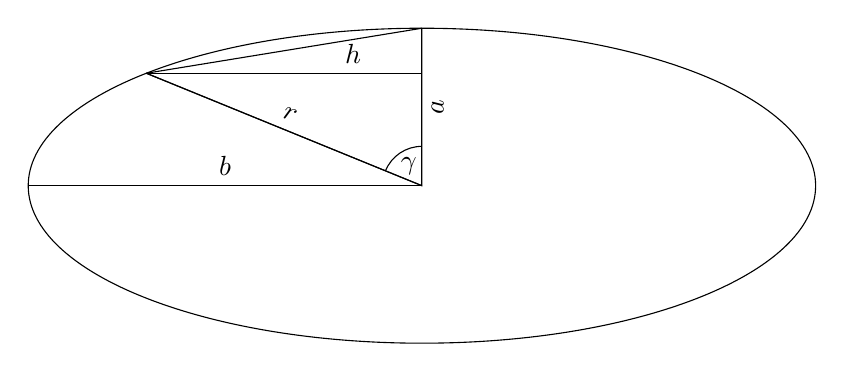
\begin{tikzpicture}
\draw (0,0) ellipse (5cm and 2cm);
\draw (-5, 0) -- (0, 0) node [midway, above] {$b$};
\draw (0, 0) -- (0, 2) node [midway, below, sloped] {$a$};
\draw (0, 0) -- (-3.5, 1.42828568570857) node [midway, above, sloped] {$r$};
\draw (-3.5, 1.42828568570857) -- (0, 1.42828568570857)  node [near end, above] {$h$};
\draw (-3.5, 1.42828568570857) -- (0, 2);
\draw (0,2) coordinate (A) -- (0,0) coordinate (B)
         -- (-3.5, 1.42828568570857) coordinate (C)
  pic ["$\gamma$", draw] {angle};
\end{tikzpicture}

\end{document}


